\documentclass[11pt]{article}
\usepackage{epsfig}    % to insert postscript figures
\usepackage{float}
\usepackage{listings}
\usepackage{url}
\usepackage{amsmath}
\parindent=0pt
\parskip=10pt
\begin{document}

\title{Optimal rotor arm pivot angles \\ for a collapsible drone.}
\author{ by \\ Peter Burnett and Hugh Murrell }
\maketitle

\newpage
\section*{Problem Description}

Consider the CAD drawing of the collapsible drone shown in figure \ref{fig1} below:

\begin{figure}[H]
\begin{center}
  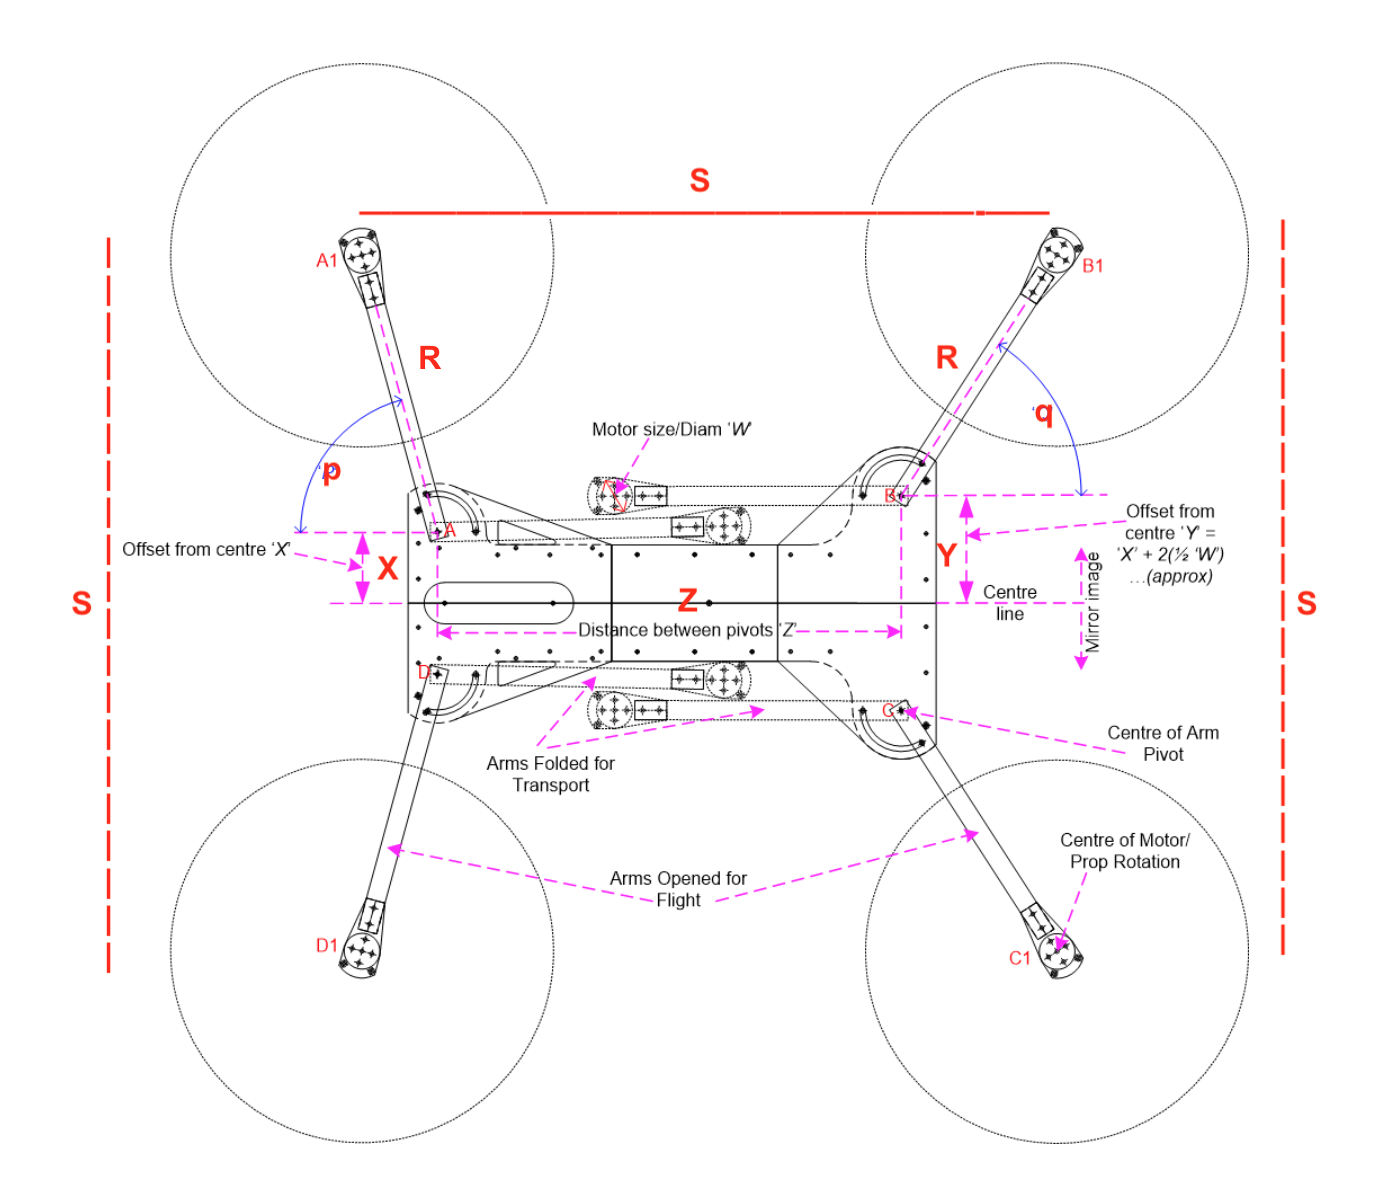
\epsfig{file=drone_drawing.png,height=3in}
\end{center}
\caption{CAD drawing of drone with collapsible arms}  
\label{fig1}
\end{figure}

In this diagram all lengths are measured in $mm$ and the annotated lengths 
are design parameters for the construction of the drone:

\begin{itemize}
\item[$R$] the length of the rotor arm (all rotor arms have the same length)
\item[$Z$] the distance between rotor arm pivot points.
\item[$X$] the offset of the front pivot arm point from the horizontal axis of symmetry.
\item[$Y$] the offset of the back pivot arm point from the horizontal axis of symmetry.
\end{itemize}

The problem is to determine the rotor arm angles, $p$ and $q$, under the
constraint that the rotor centres form a square.

\section*{Constraint Problem}

Using the constraint that the rotor centres form a square with sides of some unknown length $S$
we have:

\begin{eqnarray}
S & = & R \cos(p) + Z + R \cos(q)    \nonumber \\
S & = & 2 ( X + R \sin(p) )  \nonumber  \\
S & = & 2 ( Y + R \sin(q) )  \label{eqn1}
\end{eqnarray}

The first equation in (\ref{eqn1}) is derived from an expression for the horizontal edge of length, $S$,
whilst the last two equations are derived from expressions for the vertical front and back edges of length $S$.

The unknown edge length, $S$, can be eliminated from equations (\ref{eqn1}) yielding two non-linear
equations for the angles, $p$ and $q$ shown in equations (\ref{eqn2}) below.

\begin{eqnarray}
\cos(p) - 2 \sin(p) + \cos(q) & = & \frac{2X-Z}{R} \nonumber \\
\sin(p) - \sin(q) & = & \frac{Y-X}{R}   \label{eqn2} 
\end{eqnarray}

Although it is possible to find a closed form solution for $p$ and $q$ the calculation 
requires finding the roots of a quartic polynomial which is extremely tedious as one
can see from the Wikipedia entry \cite{quartic}.

So instead we use standard non-linear root finding technique. For example,
the {\tt scipy} python package allows us to construct the solution shown in the appendix.

To make life easier for the reader we have also coded a {\tt javascript} solution to the
problem, again using a numerical equation solver. This time we found that Martin Donk's 
{\tt javascript} library, {\tt nerdamer} \cite{donk} allowed us to compute $p$ and $q$ using
a non-linear equation solver. And we also made use of the Microsoft javascript CAD library,
{\tt Maker.js} \cite{maker}, to produce drawings dependent on the user's parameter settings. 

To access the {\tt javascript} application goto:

\url{https://hughmurrell.github.io/DroneDesign/index.html}.


\newpage
\begin{thebibliography}{99}

% \bibitem{pfund} Pfund, Michele \& Fowler, J.W. \& Gupta, Jatinder. 
% {\em A survey of algorithms for single and multi-objective unrelated parallel-machine deterministic scheduling problems}. 
% Journal of the Chinese Institute of Industrial Engineers. 21. 230-241. (2004). 

\bibitem{quartic} Wikipedia Article,
{\em Quartic function} 
\url{https://en.wikipedia.org/wiki/Quartic_function}
accessed January 2021.

\bibitem{donk} Martin Donk,
{\em nerdamer, Symbolic Math for Javascript},
\url{https://nerdamer.com/},
accessed January 2021.

\bibitem{maker} A Microsoft Garage Project,
{\em Maker.js, a JavaScript library for creating and sharing modular line drawings for CNC and laser cutters.},
\url{https://maker.js.org/},
accessed January 2021.

\end{thebibliography}

\section*{Appendix}
\subsection*{pythod code for calculating rotor arm pivot angles}

\begin{lstlisting}
from scipy.optimize import fsolve
from math import sin, cos, pi

def equations(vars):
    p, q = vars
    R = 225
    Z = 346
    X = 56
    Y = 84
    eq1 = cos(p) - 2*sin(p) + cos(q) - (2*X-Z)/R
    eq2 = sin(p) - sin(q) - (Y-X)/R
    return [eq1, eq2]

p, q =  fsolve(equations, (1, 1))

p = (p / pi) * 180
q = (q / pi) * 180

print(p, q)
\end{lstlisting}



\end{document}


